\section{Diagrama de bloques y componentes}

\subsection{Cómo está organizada la placa}

La batería es el nodo central. Dos cargadores independientes la cargan, uno desde el panel solar
(CN3791) y otro desde el USB-C (TP4056), y todo el sistema se alimenta de ella a través de un
regulador lineal de 3.3~V. El USB-C no alimenta al sistema: solo carga la batería y lleva los datos
de programación. Por eso, sin batería conectada la placa no arranca desde el USB.

\begin{figure}[H]
\centering
\resizebox{0.97\textwidth}{!}{%
\begin{tikzpicture}[
  box/.style={draw, rounded corners, align=center, font=\scriptsize, minimum height=0.9cm, text width=2.6cm},
  src/.style={box, fill=groupbg},
  core/.style={box, fill=headbg},
  >=Stealth]
\node[src] (sol) at (-6.2,2.2) {Panel solar\\6~V};
\node[src] (usb) at (-6.2,0.2) {USB-C\\5~V (y datos)};
\node[box] (cn) at (-3.1,2.2) {Cargador solar\\CN3791 (U3)};
\node[box] (tp) at (-3.1,0.2) {Cargador USB\\TP4056 (U2)};
\node[core] (bat) at (0,1.2) {Batería 1S\\3.7~V, con protección\\integrada};
\node[box] (ldo) at (3.1,1.2) {LDO 3.3~V\\TLV75733P (U4)};
\node[box] (gau) at (0,-0.9) {Medidor de batería\\MAX17048 (U9)};
\node[core] (mcu) at (7.0,3.0) {ESP32-S3\\WROOM-1U (U5)};
\node[box] (gps) at (7.0,1.8) {GNSS\\MAX-M10S (U6)};
\node[box] (lor) at (7.0,0.6) {LoRa\\DX-LR30 (U7)};
\node[box] (imu) at (7.0,-0.6) {IMU\\LSM6DS3TR-C (U8)};
\draw[->] (sol) -- (cn); \draw[->] (usb) -- (tp);
\draw[->] (cn) -- (bat); \draw[->] (tp) -- (bat);
\draw[->] (bat) -- (ldo); \draw[->] (bat) -- (gau);
\draw[->] (ldo.east) -- ++(0.35,0) |- (mcu.west);
\draw[->] (ldo.east) -- ++(0.35,0) |- (gps.west);
\draw[->] (ldo.east) -- ++(0.35,0) |- (lor.west);
\draw[->] (ldo.east) -- ++(0.35,0) |- (imu.west);
\end{tikzpicture}}
\caption{Diagrama de bloques de la alimentación y de los módulos de la PCB.}
\end{figure}

\subsection{Componentes principales}

\begin{table}[H]
\centering
\footnotesize
\begin{tabularx}{\textwidth}{|l l X|}
\hline
\tablehead{\textbf{Ref.} & \textbf{Pieza} & \textbf{Función}} \\ \hline
U5 & ESP32-S3-WROOM-1U-N16R8 & Procesador de la aplicación (Zephyr); versión con conector u.FL, sin antena impresa \\ \hline
U6 & u-blox MAX-M10S-00B & Receptor GNSS multiconstelación en L1, por UART; parche pasivo con cable y u.FL (J4) \\ \hline
U7 & DX-LR30-900M22S & Módulo LoRa con SX1262, 915~MHz, por SPI; antena de 8~cm por u.FL (J5) \\ \hline
U8 & LSM6DS3TR-C & IMU; su interrupción despierta al MCU del sueño profundo \\ \hline
U9 & MAX17048G+T10 & Medidor de carga de la batería por I2C (0x36), conectado a la batería \\ \hline
U3 & CN3791 & Cargador solar conmutado con seguimiento de punto de máxima potencia (MPPT), con L1 de 47~\textmu H \\ \hline
U2 & TP4056 & Cargador lineal desde USB-C, limitado a 500~mA \\ \hline
U4 & TLV75733PDBVR & LDO de 3.3~V, 1~A, corriente en reposo de 25~\textmu A, alimentado solo desde la batería \\ \hline
U1 & USBLC6-2SC6 & Protección ESD en D+, D$-$ y VBUS del USB-C (J1) \\ \hline
U10 & VO617A-1X017T & Optoacoplador: aislamiento galvánico del actuador \\ \hline
D3, D4, BZ1 & LED RGB, LED rojo, zumbador PS1240P02BT & Alertas visuales y sonora \\ \hline
Y1 & ECS-.327-12.5-34B-TR & Cristal de 32.768~kHz \\ \hline
\end{tabularx}
\caption{Componentes principales y su designador en el esquemático.}
\end{table}

\subsection{Hojas del esquemático}

El esquemático tiene cinco hojas: potencia y carga, microcontrolador, radio (GNSS y LoRa), sensores
(IMU y medidor de batería) e interfaz (optoacoplador, LEDs, zumbador y botón). Las páginas están en
\ruta{hardware/pcb/DR-VF-01_schematics.pdf} y se reproducen a continuación.

\foreach \p in {1,...,5}{%
\begin{figure}[p]
\centering
\includegraphics[width=\textwidth,page=\p]{DR-VF-01_schematics.pdf}
\caption{Hoja \p{} del esquemático.}
\end{figure}}
